\documentclass[twocolumn]{article}
\usepackage{fullpage}
\usepackage{amsmath, amssymb}
\usepackage{graphicx}
\usepackage{hyperref}
\usepackage{verbatim}
\usepackage{pifont}
\usepackage{authblk}
% \usepackage{natbib}

\begin{document}


\title{Evolution as Explanation:  \\The Origins of Neural Codes and their Efficiencies}
\author[1,\ding{41}]{Han Kim}
% \author[2,\ding{41}]{Po-Yi Ho}
\author[2,\ding{41}]{Zitong Jerry Wang}
\affil[1]{Fearn AI, Inc.}
\affil[2]{Center for Interdisciplinary Studies (CIS), School of Science, Westlake University, Zhejiang, China}
\affil[\ding{41}]{ \texttt{han@fearn.ai}, 
% \texttt{poyi@westlake.edu.cn}, 
\texttt{jerry@westlake.edu.cn}}

\date{\today}


\twocolumn[
  \begin{@twocolumnfalse}
    \maketitle
    \begin{abstract}
      \noindent Neural codes appear efficient. Any explanation of how nervous systems function, and of how they are organized, must nevertheless be squared with population genetics, and natural selection is only one of the forces that population genetics describes. Animals with nervous systems, and in particular those with big brains, have small effective population sizes ($N_e$), a condition under which drift is strong and natural selection is comparatively inefficient. How, then, did precise and efficient neural systems evolve in exactly these species? We survey neural systems that appear near-optimal, and argue that they point to selection strong enough to overpower drift. We contrast them with the variation found beneath conserved neural phenotypes: degenerate biophysical parameters, homologous neurons that play different circuit roles, turnover of receptor genes, and divergent gene expression in conserved cell types. We propose that both observations follow from a layered genotype-phenotype map, in which the neural or behavioural phenotype is held in place by strong stabilizing selection, while the layers beneath it are free to drift, much as in developmental systems drift. A computational model of organisms as layered systems shows that layers buffer genetic perturbation and accelerate convergence to fitness optima, even for small $N_e$ species. We advocate for a pluralistic neuroscience capable of appealing to both adaptive and non-adaptive evolutionary explanations.
    \end{abstract}
    \vspace{1.5em}
  \end{@twocolumnfalse}
]




\section{Introduction}

Neural codes appear efficient. Across sensory, motor, and central systems, neuroscientists have found codes and circuits that seem to approach the best possible solution to the problem at hand, in some cases, right up to the limits imposed by physics \cite{barlow_1952, Barlow_1961, simoncelli_olshausen_2001}. The efficient coding hypothesis has turned this observation into one of the most productive frameworks in neuroscience \cite{Barlow_1961, barlow_2001, simoncelli_olshausen_2001}. Intuitively, an efficient process appears responsible for generating efficient codes, and natural selection is oft cited as that process.

Any explanation of how nervous systems function, and of how they are organized, must ultimately be squared with population genetics. Evolution is not natural selection. Rather, it consists of four forces, of which natural selection is just one. The other three---mutation, recombination, and genetic drift---are non-adaptive, because they are random and do not depend on an animal's fitness. Natural selection is an important force, but the extent to which it, by itself, explains the organization of brains and neural circuits remains unclear.

In fact, the features of nervous systems that impress us the most---the apparent precision and efficiency of neural circuits---appear to have evolved in the face of a marked inefficiency of natural selection. Animals with nervous systems, and in particular, those with big and powerful brains, have the smallest effective population sizes of any organisms \cite{Lynch_Conery_2003}. In such populations, drift is strong and selection is comparatively weak, and the genomes of these species bear the marks of features that natural selection could not purge \cite{Lynch_2007}. How, then, did efficient neural codes arise in exactly those species where natural selection is least efficient? And why, in the same species, do other neural features vary freely between individuals and species, or even appear suboptimal?

In this paper, we attempt to resolve this conundrum. We first outline, briefly, the population genetics that make the efficiency of neural codes surprising. We then survey two sets of neurobiological examples: neural systems that appear near-optimal, and neural systems that vary without apparent consequence for function. We argue that both sets of observations make sense under a layered view of the genotype-phenotype map. In this view, the neural or behavioural phenotype, which interacts most directly with the environment, is under strong selection, but it can be generated by many alternate configurations of the layers beneath it---ion channel densities, gene expression programs, circuit wiring---which are consequently free to drift.

We must posit, in other words, that certain neural phenotypes are so strongly adaptive that they are selected for, and held in place by purifying selection, despite small effective population sizes. Where the efficiency of a neural system is undeniable, it points to a fitness advantage so large that it overpowers the exceptionally strong drift that pervades genome evolution in these species. Beneath that anchored phenotype, however, evolution can be far more dynamic. This idea is not new to biology. Developmental biologists have long documented phenotypes that are maintained by strong stabilizing selection, even as the genetic and cellular mechanisms that build them turn over between species \cite{True_Haag_2001, Parker_Pennell_2025}. We contend that nervous systems are analogous. We formalize this view with a computational model of organisms as layered systems, and we close in support of a pluralistic neuroscience that accommodates both adaptive and non-adaptive explanations.

\section{Small effective population sizes weaken natural selection} \label{sec_popgen}

Under what conditions, then, will non-adaptive forces outweigh natural selection? The goal of this section is, in part, pedagogical. We aim to explain the key population genetic concepts, without being mired by technical derivations, and we point the interested reader to more thorough treatments \cite{Lynch_2007, charlesworth_2009}.

The answer depends largely on a parameter that Sewall Wright called the effective population size, $N_e$ \cite{wright_1931}. Each generation of a population is, in effect, a random sample of the genetic material of the generation before it. The smaller the population, the larger the sampling error, and the more allele frequencies change by chance alone---that is, by genetic drift. $N_e$ is the size of an idealized population that would experience the same amount of drift as the real one. In other words, it measures how strongly chance acts on a population. For nearly all species, $N_e$ is far smaller than the actual number of breeding individuals \cite{crow_newton_1955, frankham_1995, lynch2007origins}.

Natural selection can only act on a genetic variant if that variant's effect on fitness is large, relative to the strength of drift. When a variant's selective advantage or disadvantage is smaller than roughly the inverse of $N_e$, the variant behaves as though it were neutral. Its fate is decided by chance and by mutation pressure, rather than by its consequences for the organism \cite{kimura1983neutral, Lynch_2007, lynch_hagner_2015}. Slightly beneficial variants can be lost, and slightly deleterious variants can fix. The smaller the $N_e$, the larger the class of variants to which natural selection is effectively blind.

Which species, then, possess small effective population sizes? Estimates derived from neutral genetic diversity place $N_e$ at $10^8$ or more for prokaryotes, $10^7$ to $10^8$ for unicellular eukaryotes, $10^5$ to $10^6$ for invertebrates, and $10^4$ to $10^5$ for vertebrates \cite{Lynch_Conery_2003}. Animals with nervous systems have the smallest values, and vertebrates, including the species with the biggest brains, have smaller values still. Lynch has argued that these differences explain much of the architecture of eukaryotic genomes \cite{Lynch_2007, lynch2007origins}. Prokaryotic genomes are compact and almost entirely protein-coding, whereas the genomes of multicellular eukaryotes are bloated with introns, non-coding sequence, and pervasive transcription whose products are mostly degraded \cite{milo2016cell, menet_rosbash_2012, mcnicoll_neugebauer_2014}. These features need not be adaptations. They are, at least in part, what accumulates when natural selection is too weak to remove them \cite{Lynch_2007}.

We emphasize that the small $N_e$ of nervous system-possessing animals does not make them impervious to natural selection. Rather, it raises the bar. For natural selection to have produced, and to maintain, a given trait in these species, the fitness consequences of that trait must be large. As we will see, many neural systems clear this bar with room to spare.

\section{Efficient codes across the nervous system} \label{sec_efficient}

If small effective population sizes weaken natural selection, then we might expect abundant inefficiencies across the nervous systems of animals. This expectation, however, appears to be exceptionally false. In this section, we survey neural systems that appear near-optimal, sometimes to the point of physical limits. We contend that these cases are best explained by natural selection, and moreover, that they point to selection of unusual strength.

\subsection{Sensory systems}

The clearest case is perhaps also one of the oldest. A survey of ommatidia diameter and eye height from 27 \textit{Hymenoptera} species suggests that their facets have evolved to maximize visual sampling, while minimizing the blur from diffraction \cite{barlow_1952}. This conclusion derives from a fundamental physical principle: the optimal resolving power of a lens with diameter $d$ is proportional to $\sqrt{a\lambda}$, where $a$ is the angle subtended by two point sources that can still be detected as double, and $\lambda$ is the wavelength of incoming light. The surveyed insects indeed possess a linear and proportional relationship between $\sqrt{a}$ and $d$ \cite{barlow_1952}. What is striking about this result is not only that the insect eye sits at the optimum, but that we do not see eyes that deviate from it. Facets that are slightly too small or too large must cost their owners dearly, such that the individuals that possess them are purged from the population before they can be observed, within or between species.

The vertebrate rod photoreceptor tells a similar story. Human observers can detect a flash of light from which rods absorb only a handful of photons, and a single photon is sufficient to excite a single rod \cite{Hecht_Shlaer_1942}. Recordings from toad rods later confirmed that a single photoisomerization produces a reliable electrical response \cite{Baylor_Lamb_1979, Rieke_Baylor_1998}. Light arrives in discrete quanta, and so the rod operates at the limit of what is physically possible. Several other sensory systems appear to operate near such limits \cite{Bialek_1987}.

Efficiency extends from the detection of signals to their encoding. In the fly compound eye, the contrast-response function of the first-order interneurons closely approximates the cumulative distribution of contrasts in natural scenes---exactly the function that information theory predicts will make the best use of the neuron's limited response range \cite{Laughlin_1981}. In feline, human, and grasshopper auditory systems, neurons appear to use a sparse spike code to represent acoustic stimuli, and kernel functions for an optimal sparse representation learned from natural sounds closely approximate the physiological reverse-correlation filters \cite{Machens_Gollisch_Kolesnikova_Herz_2005, smith_lewicki_2006}. Importantly, these codes succeed only when the stimulus derives from natural scene statistics, and they are especially tuned for behaviourally relevant stimuli \cite{Machens_Gollisch_Kolesnikova_Herz_2005, machens_herz_2001}. In the retina, the ganglion cells of both salamanders and macaques decorrelate spatial features of visual inputs, as a means of achieving sparse spiking and optimizing coding efficiency \cite{Pitkow_Meister_2012}.

\subsection{Wiring and energy}

Efficiency is not limited to the periphery. In \textit{C. elegans}, the placement of the ganglia minimizes the total length of the connections between them: of the roughly 40 million possible orderings, the observed layout is the one with the least total wire \cite{Cherniak_1994}. At the level of single neurons, an optimal layout that minimizes wiring places most of the worm's neurons close to their actual positions \cite{Chen_Hall_2006}. Underlying these results is the fact that neural signalling is expensive. In the blowfly retina, transmitting a single bit of information costs between $10^4$ and $10^7$ molecules of ATP, depending on the pathway \cite{Laughlin_deRuyterVanSteveninck_1998}, and much of the brain's energy budget is spent restoring ion gradients after signalling \cite{sengupta_2010, Niven_Laughlin_2008}. Energy, in other words, is a currency that selection can see, and many neural systems appear to spend it frugally \cite{Niven_Laughlin_2008}.

\subsection{Motor and central systems}

Some evidence suggests that the encoding of naturalistic behaviours also has an efficient basis. Simultaneous microdrive recordings and 3D posture tracking of freely moving rats reveal that proportionately fewer cells in posterior parietal and motor cortices fire when the animal adopts common `default' postures \cite{Mimica_Dunn_Tombaz_Bojja_Whitlock_2018}. The encoding of naturalistic poses appears to use a minimal number of cells to represent the repertoire of ethological motor ensembles. Further examples of efficiency have been argued in deeper processing regions, albeit often with different, and arguably more ambiguous, objectives from the sparse coding seen at the periphery \cite{simoncelli_2003}. Learning algorithms that maximize sparseness, for example, succeed in recapitulating the spatially localized, oriented, and bandpass features of mammalian visual cortical cells \cite{olshausen_field_1996}, and sparse codes in the visual cortex appear useful for parsing signal from noise \cite{ringach_malone_2007}.

\subsection{Near-optimality points to strong selection}

An appeal to natural selection as the process behind these findings is not problematic. In fact, it is likely the most appropriate explanation. We wish, however, to make explicit what such an appeal requires, given the population genetics of Section~\ref{sec_popgen}. For a phenotype to sit at an optimum in a species with a small $N_e$, the fitness cost of deviating from that optimum must be large enough to overpower drift. Near-optimality in these species is therefore not merely consistent with natural selection. It is evidence that the phenotype in question confers an extremely strong adaptive advantage, and that it is held in place by purifying selection that removes deviants as fast as they arise. The insect eye, the rod photoreceptor, and the wiring of the worm are, in this sense, the visible signature of very strong selection.

This conclusion, however, leaves us with a puzzle. If the precision of these systems requires such strong selection, and if selection is otherwise weak in these species, then what of everything else in the nervous system? We turn to this question in the next section.

\section{Variation beneath conserved neural phenotypes} \label{sec_variation}

Alongside the near-optimal systems above, neuroscientists have documented a striking amount of variation, both between individuals and between species, in the cellular and molecular parameters that generate neural function. In many of these cases, the variation appears to have no consequence for the phenotype that the parameters generate. In this section, we survey such cases. We argue that they are what one would expect if the higher-level neural phenotype is held in place by strong selection, while the lower levels that generate it are free to drift.

\subsection{Degenerate parameters in the stomatogastric ganglion}

The crustacean stomatogastric ganglion consists of a small and defined network of neurons that fire in a precisely ordered and periodic manner, producing the pyloric rhythm that enables the animal to digest food. The simulation of more than 20 million versions of a model pyloric network reveals that nearly identical network activity can arise from widely disparate combinations of synaptic and intrinsic parameters \cite{prinz_marder_2004}. In other words, the same network phenotype can be multiply realized. Real animals appear to take advantage of this freedom. In identified neurons of the crab stomatogastric ganglion, the conductances of three potassium currents, and the expression of the mRNAs that encode them, vary two- to four-fold from one animal to the next \cite{Schulz_Goaillard_2006}, and yet each animal produces a functional pyloric rhythm (Figure \ref{fig_examples}).

For the neuroscientist limited to the powers of natural selection, the origins of this wanton degeneracy are not straightforward to explain. A layered view of phenotype, however, accommodates it easily. Biophysical parameters can afford to vary, provided that they generate the network dynamics required for organismal function. The biophysical level is free to drift, while the network level above it remains under selection.

\subsection{Homologous neurons, similar behaviours, different circuits}

If lower levels drift beneath a conserved phenotype within species, we might expect them to diverge between species that share the same phenotype. The nudibranch molluscs \textit{Melibe} and \textit{Dendronotus} swim in the same way, with rhythmic left-right flexions of the body, and their swim circuits contain homologous, individually identifiable interneurons. Yet the homologous neurons do not play the same roles. One interneuron, Si1, is a member of the swim central pattern generator in \textit{Melibe}, but not in \textit{Dendronotus} \cite{Sakurai_Newcomb_2011}. The behaviour is conserved, the cells are conserved, but the circuit that connects them to the behaviour is not (Figure \ref{fig_examples}). Even the wiring between homologous neurons can be remarkably labile. Every pharyngeal neuron of the nematode \textit{Pristionchus pacificus} has a homologue in \textit{C. elegans}, but the connections between them have been extensively rewired \cite{Bumbarger_Riebesell_2013}. In this case, the behaviour differs between the two species, and so the rewiring cannot be attributed to drift alone, but it demonstrates how freely the circuit level can change while cell identities are conserved.

A related pattern appears when distantly related animals arrive at the same computation. Barn owls and mammals both localize sounds using the minute differences in the arrival time of sounds at the two ears, but they appear to do so via different neural mechanisms: delay lines in birds, and precisely timed inhibition in mammals \cite{Grothe_2003, McAlpine_Grothe_2003}. Because these mechanisms likely evolved independently, this is a case of convergence rather than drift. It nevertheless conveys the same lesson: selection can be very particular about what a neural system computes, and indifferent to how it is computed. Even at the motor periphery, the songbird vocal organ can produce the same acoustic output from more than one combination of motor commands \cite{Elemans_Rasmussen_2015}, leaving room for the motor level to vary beneath a conserved song.

\subsection{Turnover of genes and cell-type expression}

Beneath circuits lie the genes that build them, and here, the evidence for drift is clearest. The chemosensory receptor gene families of animals are among the most dynamic in the genome. Their sizes vary enormously between species, and much of this variation appears to result from random gene duplication and deletion---a process that Nei and colleagues term `genomic drift'---rather than from adaptation to particular chemical environments \cite{Nei_Niimura_2008}. Gene copies born neutrally can nevertheless become substrates for later adaptation. An ancient duplicate of a muscle sodium channel gene, retained since the genome duplication at the base of the teleost fishes, was co-opted more than 100 million years later for the electric organs of two independent lineages of electric fish \cite{Arnegard_Zwickl_2010}. For many macroevolutionary processes, the outcomes of neutral events can be co-opted in this way \cite{Lynch_2007, bruckner_2021, kebschull_luo_2020}.

At the level of cell types, single-cell transcriptomics now allows the comparison of homologous neurons across species at the resolution of their entire expression profiles. A comparison of human and mouse cortex finds that cell types are well conserved and can be matched between the two species, yet homologous types differ in their proportions, laminar distributions, morphologies, and in the expression of many genes \cite{Hodge_Bakken_2019}. The identity of the cell type, which is what the circuit presumably requires, is conserved. Much of its molecular composition is not.

\subsection{Entrenchment: the inverted vertebrate retina}

Not every apparent inefficiency in the nervous system is the product of drift. The vertebrate retina is inverted: light must pass through the ganglion cells, the inner synaptic layer, the amacrine, bipolar, and horizontal cells, and the outer synaptic layer, before it reaches the photoreceptive rods and cones \cite{sterling_laughlin_principles, land_nilsson_2012}. This arrangement scatters incoming light, and because the axons of the ganglion cells must exit the eye through the photoreceptor layer, it produces a literal blind spot. The everted retinas of cephalopods, spiders, and several invertebrate phyla demonstrate that the alternative is possible \cite{land_nilsson_2012, norgaard_2008, richter_2010, garm_2010}. The inverted retina, however, is best understood as a case of historical entrenchment rather than drift. It likely reflects an arrangement that was an improvement over its predecessor at the time it arose, and that subsequent evolution, constrained by everything built upon it, could not easily undo. Entrenchment is also a historical, non-adaptive explanation, but it is a different one from drift, and we mention it here to avoid conflating the two. Functional arguments for the inverted design \cite{kroger_2009} are, in our view, better read as accounts of how vertebrates have compensated for an entrenched arrangement, than as accounts of why it exists.

\subsection{Speculations across clades}

Finally, we note two comparisons between vertebrates and invertebrates that are consistent with, but by no means demonstrate, a greater contribution from drift in the smaller $N_e$ vertebrates. Vertebrate neurons are typically multipolar, integrating their inputs at the cell body before producing a single output \cite{hu_bean_2018, kandel2013principles}, whereas invertebrate neurons are typically unipolar, and can multiplex several computations in spatially separate compartments of a single neurite \cite{watson_burrows_1985, Hendricks_Ha_Maffey_Zhang_2012}. And brainwide recordings reveal that ongoing behaviour is represented redundantly across much of the vertebrate brain, including primary sensory areas, whereas the sensory neurons of \textit{C. elegans} do not participate in this representation \cite{stringer_harris_2019, kato_2015, kaplan_zimmer_2020, aimon_2019, schaffer_2021}. These comparisons are confounded by many differences besides $N_e$, and we offer them only as speculations worth testing.

\begin{figure*}[htp]
\centering
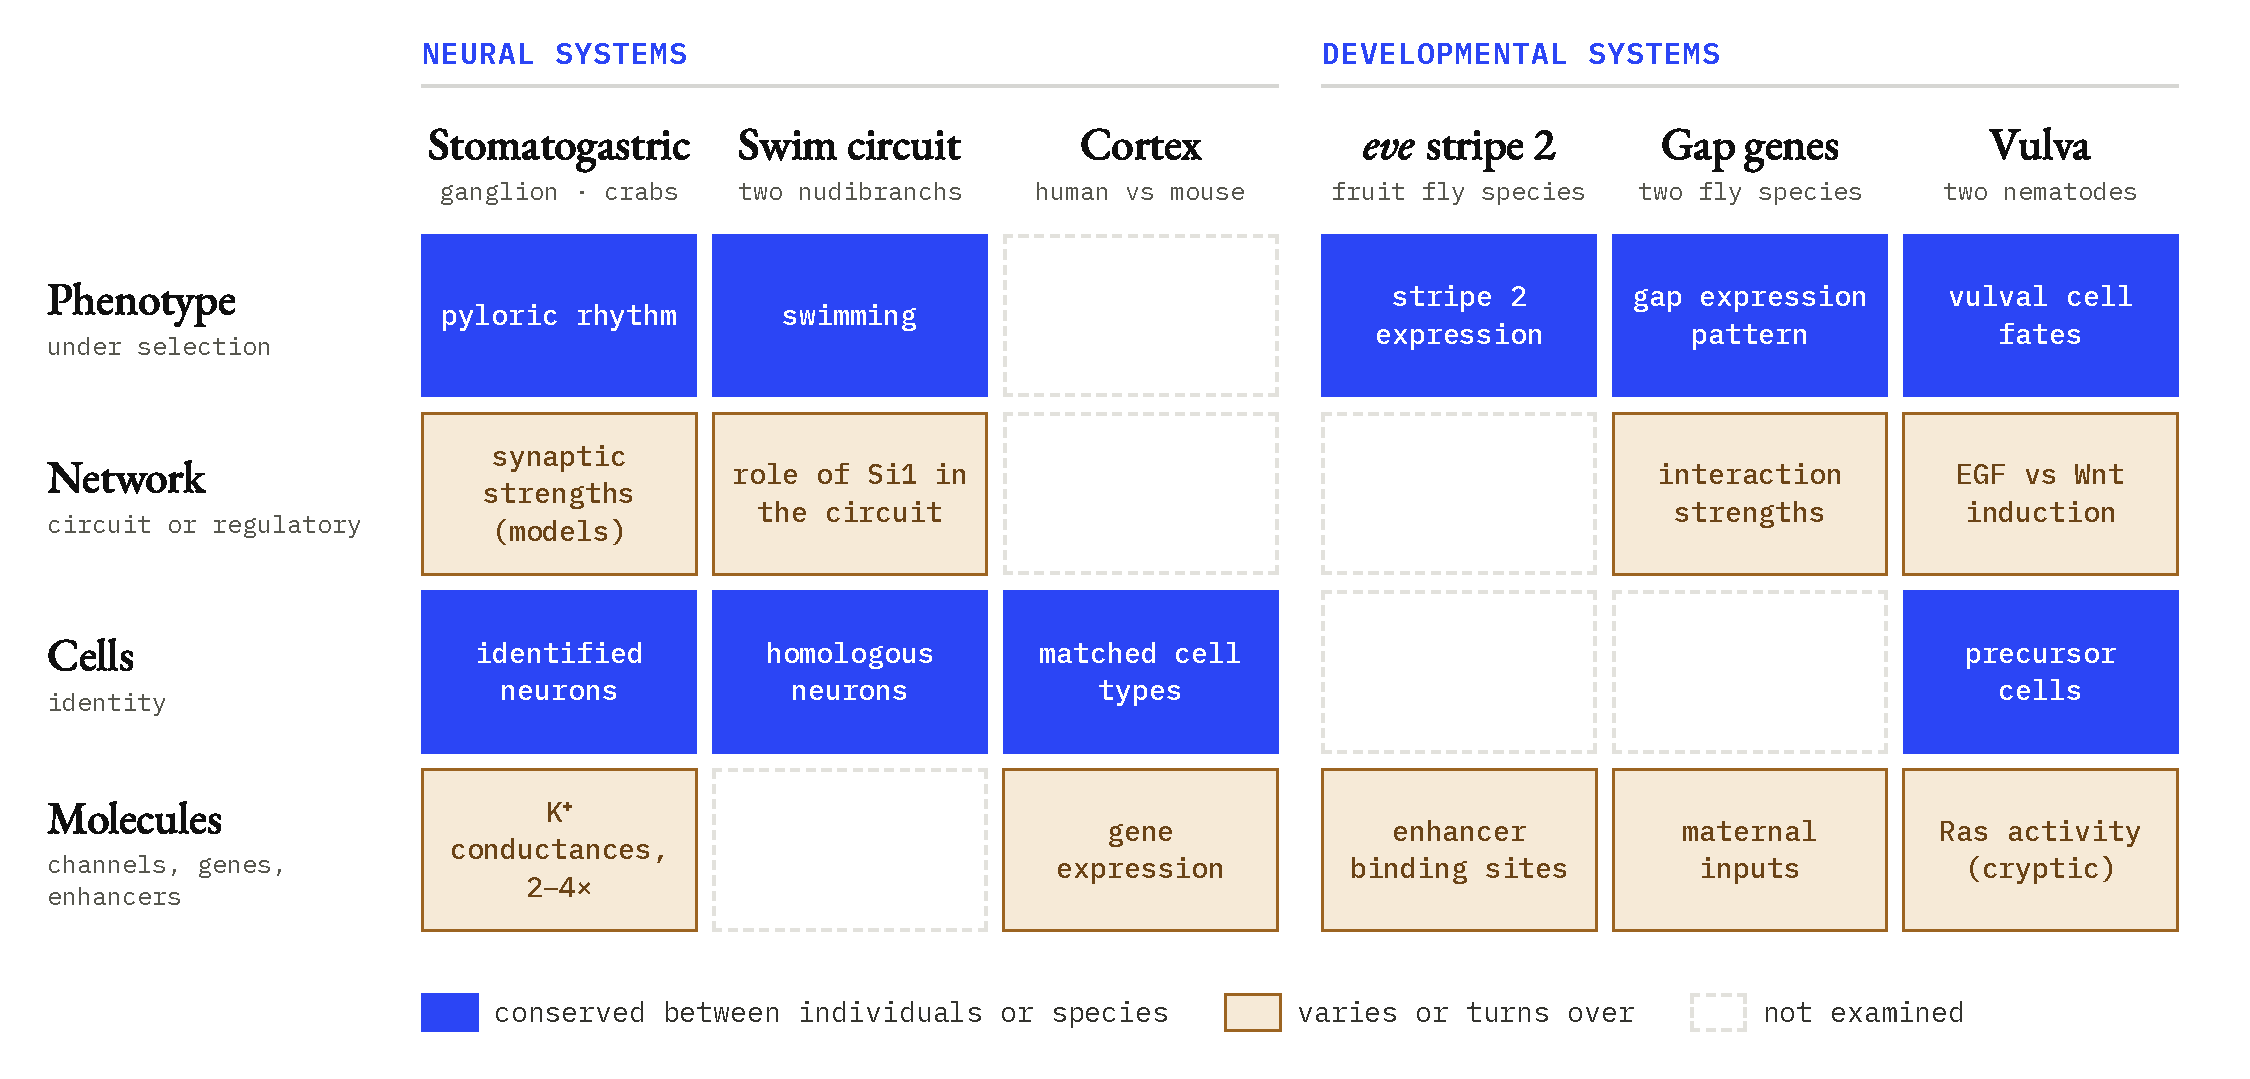
\includegraphics[width=\textwidth]{fig_layers.pdf}
\caption{\textbf{Phenotypes held in place by selection, above layers that vary.} Each column is an example from the text; each row is a layer of phenotype, from the phenotype under selection down to its molecular basis. Blue: conserved between individuals or species. Ochre: varies between individuals or species, or turns over during evolution. Dashed: not examined in the cited work. Neural systems: the pyloric rhythm of the crab stomatogastric ganglion, produced by identified neurons whose potassium conductances vary two- to four-fold between animals \cite{Schulz_Goaillard_2006}, and by disparate synaptic strengths in models \cite{prinz_marder_2004}; swimming in the nudibranchs \textit{Melibe} and \textit{Dendronotus}, where homologous neurons play different roles in the swim circuit \cite{Sakurai_Newcomb_2011}; and human and mouse cortical cell types, matched across species but divergent in gene expression \cite{Hodge_Bakken_2019}. Developmental systems: stripe 2 of \textit{even-skipped} expression, conserved over divergent enhancer binding sites \cite{Ludwig_Bergman_2000}; the gap gene pattern of \textit{Megaselia} and \textit{Drosophila}, reached through different maternal inputs and interaction strengths \cite{Wotton_JimenezGuri_2015, Crombach_Wotton_2016}; and the nematode vulva, induced by EGF signalling in \textit{C. elegans} and Wnt signalling in \textit{P. pacificus} \cite{Tian_Schlager_2008}, with cryptic variation in Ras activity within \textit{C. elegans} \cite{Milloz_Duveau_2008}.}
\label{fig_examples}
\end{figure*}

\section{A model of layered phenotypic evolution}

The examples above reveal a pattern. Where a neural phenotype interacts directly with the environment, and where its efficiency is plain, we find evidence of strong selection. Beneath such phenotypes---in biophysical parameters, circuit wiring, gene repertoires, and the expression profiles of cell types---we find variation that appears to have little consequence for function. In this section, we argue that this pattern follows from the layered organization of phenotypes, and we formalize the argument with a computational model.

\subsection{Phenotypes as a hierarchy}

Most accounts of evolution express themselves in genetic terms. In the population genetics of Section~\ref{sec_popgen}, for example, natural selection and drift act on alleles, and a biological trait's prevalence in a population is described through the fixation of its underlying alleles. In reality, however, one or two genes rarely encode for a phenotype, and theorizing about gene fixation dynamics is not identical to theorizing about the fixation dynamics of the phenotypes those genes contribute to. The central dogma of molecular biology \cite{crick_1970} explains how genetic material encodes for proteins, but it does not explain how those proteins encode for organismal function. Even Motoo Kimura, the founder of neutral theory, speculated that the relevance of neutral theory is likely minimal with respect to phenotypic evolution \cite{kimura1983neutral, kimura2020my, Zhang_2018}.

We propose the divvying of phenotypes into constituent `layers' \cite{Ho_Ohya_Zhang_2017, mayr_1997, wideman_doolittle_2019, Zhang_2018}. Elements of a lower layer can afford to vary or drift, provided that their effects do not impinge on the integrity of the layer directly above. In other words, intermediary layers `buffer' the effects that bottom layers have on the highest layers, such as animal fitness. Natural selection acts directly on phenotype, rather than genotype \cite{mayr_1997}, and so change occurring at a layer to which selection is blind will be neutral, provided that it does not affect the layer above \cite{mayr_1997, wideman_doolittle_2019, Zhang_2018}. The probability of a given change being neutral is greater, the lower the layer of the change. The relative contribution of natural selection is, in this view, a function of two parameters: the effective population size, and the layer at which variation is observed (Figure \ref{fig_framework}).

\begin{figure}[htp]
\centering
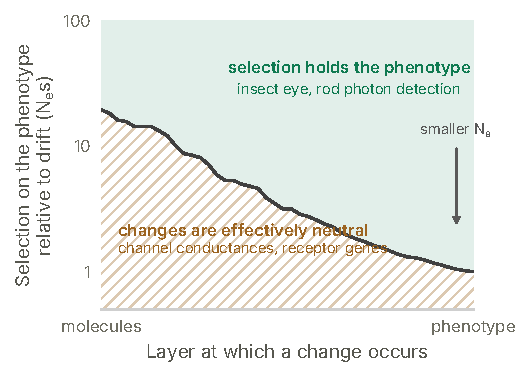
\includegraphics[width=\columnwidth]{fig_framework.pdf}
\caption{\textbf{Where selection can see a change.} A change at a given layer reaches the phenotype under selection only after passing through the layers above it, which attenuate its effect. Selection can act on the change only when the strength of selection on the phenotype, relative to drift ($N_e s$), multiplied by this attenuation, exceeds roughly one; otherwise the change is effectively neutral. The boundary uses the attenuation measured in our model (Figure \ref{fig:model_1}B), and is illustrative rather than quantitative. Phenotypes under very strong selection, such as the facets of the insect eye or the photon sensitivity of rods, are held in place even in species with small $N_e$, while changes deep beneath them, such as in channel conductances or receptor genes, can drift. A smaller $N_e$ lowers $N_e s$, and so enlarges the region in which changes are effectively neutral.}
\label{fig_framework}
\end{figure}

\subsection{Precedents in developmental biology}

This view of phenotypes is not new to biology, and developmental biologists have documented it extensively. True and Haag coined the term `developmental system drift' for the observation that homologous characters, conserved between species, are often built by divergent developmental and genetic mechanisms \cite{True_Haag_2001, McColgan_DiFrisco_2024}. In \textit{Drosophila}, the second stripe of \textit{even-skipped} expression is conserved across species, even though the binding sites within the enhancer that drives it have diverged. Chimeric enhancers, built from halves of different species' sequences, fail to drive normal expression, which suggests that the divergence is not neutral at the level of the sequence, but is compensated, such that the expression pattern itself is held in place by stabilizing selection \cite{Ludwig_Bergman_2000}. The gap gene network that patterns the fly embryo shows the same behaviour on a larger scale. The scuttle fly \textit{Megaselia} receives different maternal inputs from those of \textit{Drosophila}, yet its gap genes converge on an equivalent pattern through compensatory changes in the strengths of regulatory interactions \cite{Wotton_JimenezGuri_2015, Crombach_Wotton_2016}. The nematode vulva is perhaps the best-studied case. In \textit{C. elegans}, wild isolates produce the same pattern of vulval cell fates, but harbour cryptic variation in the signalling network that induces them \cite{Milloz_Duveau_2008, Felix_Wagner_2008}. In \textit{Pristionchus pacificus}, the same organ is induced by an entirely different signalling pathway \cite{Tian_Schlager_2008}.

Parker and Pennell have recently extended this logic to the evolution of cell types \cite{Parker_Pennell_2025}. They argue that what makes cells `visible' to natural selection is not individual genes, but gene expression programs: sets of co-expressed transcripts that collectively encode a cellular subfunction. Selection preserves the phenotypic output of a program, even as the transcripts that compose it are gained and lost. We contend that nervous systems are analogous (Figure \ref{fig_examples}). The pyloric rhythm, the swim of a nudibranch, and the identity of a cortical cell type are each conserved outputs, maintained by stabilizing selection, beneath which the parameters, circuits, and genes that generate them are free to turn over.

\subsection{Why neural codes can be efficient}

This framework explains the efficiency of neural codes, despite small $N_e$. The fact that most evidence for efficient coding relates to peripheral sensory processing and to the control of naturalistic behaviour is likely not a coincidence. Neural codes instantiated in these systems interact directly with the native environment, and by extension, with selective forces. Indeed, in the case of the optimal \textit{Hymenoptera} ommatidia \cite{barlow_1952}, the efficient implementation is not neural, but has in common an apparatus that routinely interacts with the environment. The relevant parameter is proximity to the phenotype under selection, rather than it being neural, \textit{per se}. For this reason, the framework applies broadly to phenotypic attributes beyond nervous systems. That being said, we argue that it is of special relevance to neuroscience, because of the unusual success that an optimization-based worldview has had for the field.

\subsection{A computational model}

We now test this framework computationally. We model an organism as a layered system, where a `lower' layer encodes the layer immediately above via a linear function. We show that layered organisms are 1) more robust to perturbations, and 2) more likely to possess efficient phenotypes over evolutionary time, compared to organisms without layers. The rate at which a species finds the fitness optimum increases sublinearly with the number of layers, suggesting that the accrual of layers may eventually itself be subject to drift. Hence, species in nature are unlikely to possess an alarmingly high number of layers.

Our model consists of two processes. The first determines how information at the lowest layer propagates to determine phenotypes at higher layers (\autoref{fig:model_1}A). The second determines how the species population changes across generations (\autoref{fig:model_2}A). We represent each individual $i$ by its phenotype at $N$ different layers, where $x_l^i \in \mathbb{R}^n$ denotes its phenotype at layer $l$. The lowest layer, $l=0$, represents the genotype, and the highest layer, $l=N$, represents fitness. Each subsequent layer is a linear function of the layer below,
\[ x_{l+1}^i = M_{l}x_l^{i}.\]
The linear maps, $M_l \in \mathbb{R}^{n \times n}$, are random Gaussian matrices with independent entries sampled as
\[
(M_l)_{ij} \sim \mathcal{N}(0, \sigma^2).
\]
We interpret these maps as developmental processes that propagate information from one layer to the next. These processes are influenced by the environment. Each environment has a different set of randomly sampled transformations, $\{M_l\}_{l=0}^N$.

We combine this with classical evolutionary dynamics (\autoref{fig:model_2}A). We impose natural selection on the highest layer and mutation on the lowest. A population of $M$ organisms has fitness $\{x_N^i\}_{i=1}^{M}$, where $x_{\text{opt}}$ is the optimal fitness vector with unit length. An individual's selection probability, $p_i$, (red vector in \autoref{fig:model_2}A) is
\[p_i \propto x_N^i \cdot x_{\text{opt}}.\]

Natural selection favours organisms with fitness vectors similar in direction to the optimal fitness vector, which is randomly generated but fixed for each environment. Selection, in our model, acts only on the highest layer, in keeping with our argument that it is the phenotype interacting with the environment that is held in place by selection, while the layers beneath it are free to vary.

Offspring genotypes are obtained by sampling with replacement, with probabilities $\{p_i\}^M$, maintaining constant population size. Mutation is simulated by adding Gaussian noise to each sampled genotype:
\[
x_0^i \leftarrow x_0^i + \epsilon, \quad \epsilon \sim \mathcal{N}(0, s^2).
\]
This cycle of selection and mutation then repeats \textit{ad infinitum}.

\begin{figure}[!ht]
\centering
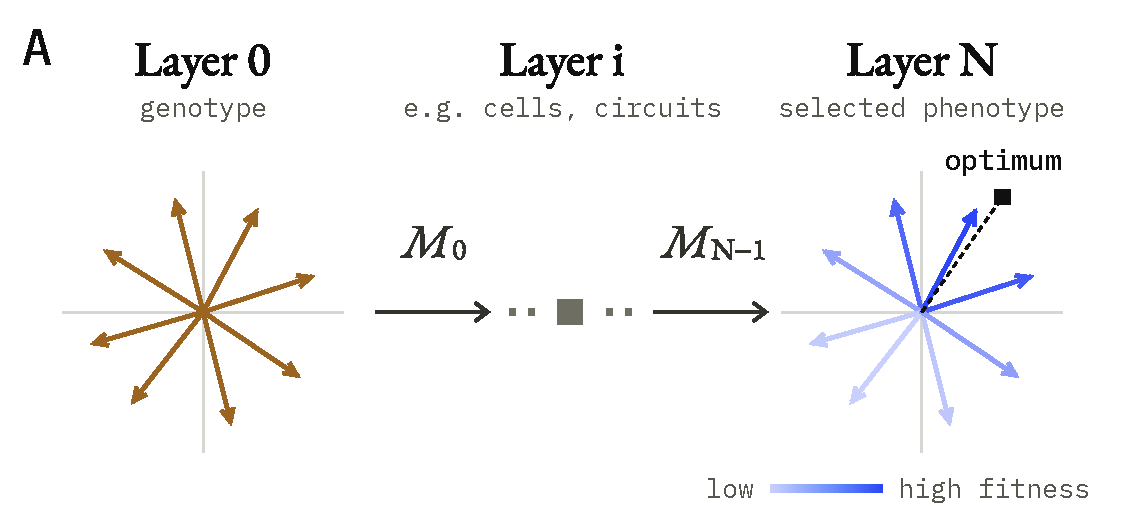
\includegraphics[width=\columnwidth]{fig_model_a.pdf}\\[4pt]
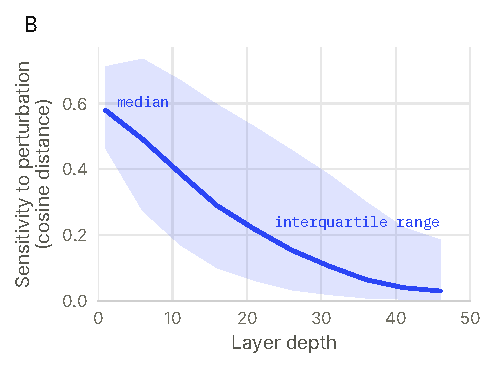
\includegraphics[width=\columnwidth]{fig_model_b.pdf}
\caption{\textbf{A model representing hierarchy of phenotype.} A) Population represented by a collection of $n$-dimensional vectors. The layer $0$ phenotype, e.g., genetic information, propagates to determine a higher layer phenotype, via random linear maps ($M_i$), up until the final layer, e.g., the fitness layer. Fitness of an individual is defined as the cosine similarity between the individual's vector at layer N and the optimal fitness vector (re-scaled to be between $0$ and $1$). B) The effect size or `sensitivity' at the various layer depths, in response to a random perturbation at the lowest layer, for species with 50 layers. Sensitivity is measured across 25 randomly generated layered systems, each perturbed with 10,000 random inputs. The line traces the median, and the shading represents the first to third quartile.}
\label{fig:model_1}
\end{figure}

\begin{figure*}[t]
\centering
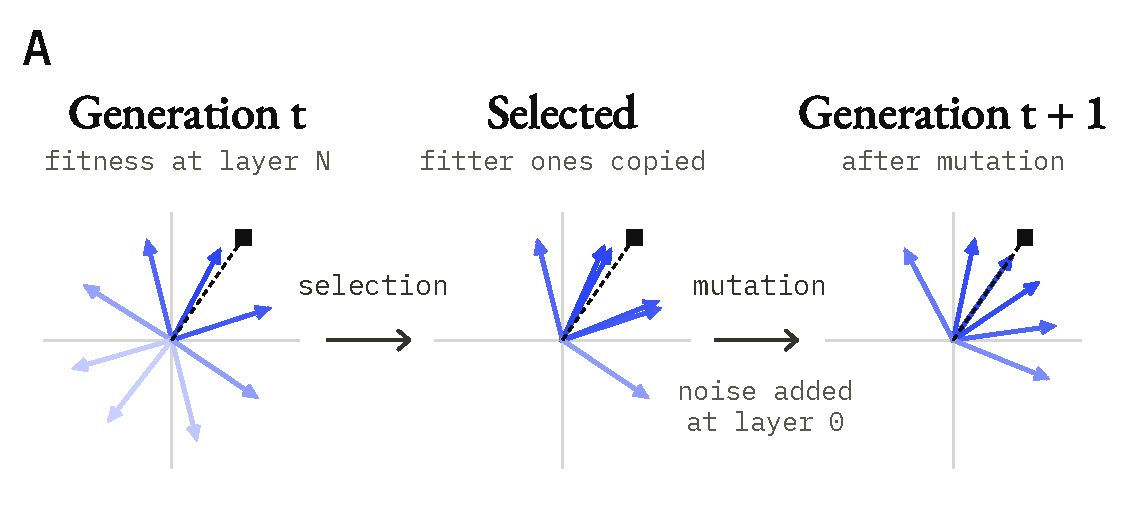
\includegraphics[width=\columnwidth]{fig_sim_a.pdf}\\[6pt]
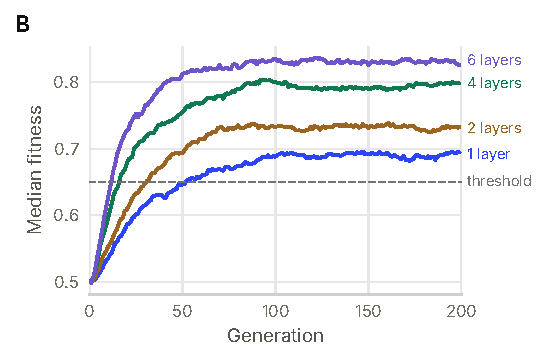
\includegraphics[width=\columnwidth]{fig_sim_b.pdf}\hfill
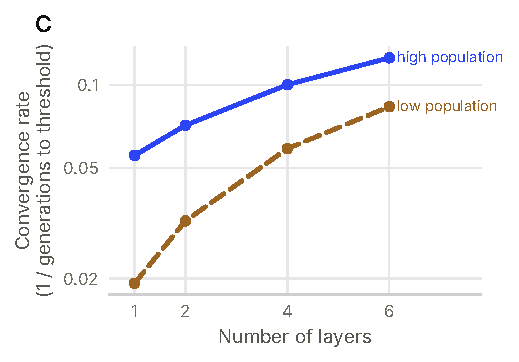
\includegraphics[width=\columnwidth]{fig_sim_c.pdf}
\caption{\textbf{Simulating evolution across hierarchy of phenotype.} A) In our evolution model, selection probability is higher for vectors that are closer to the optimal vector (black square), in terms of fitness layer, followed by mutation occurring at layer $0$ of the selected individuals. B) Median fitness over generations for organisms with different numbers of phenotypic layers, in a population of 5 individuals, across 640 runs. The dashed line at a median fitness of 0.65 indicates the threshold used in C. C) The convergence rate---the inverse of the number of generations needed to reach a median fitness of 0.65---for species with different numbers of layers, in populations of 5 (low) and 75 (high) individuals.}
\label{fig:model_2}
\end{figure*}


\subsection{Results}

Our model reveals two key results. First, when an organism is perturbed at the lowest layer, higher-layer phenotypes are more robust to the perturbation than any layers underneath (Figure~\ref{fig:model_1}B). The perturbation is a Gaussian noise injection at $l=0$, and the sensitivity is the cosine distance between the perturbed and unperturbed vectors at each higher layer. Lower layers exhibit greater cosine distance---greater sensitivity---than higher layers. In biological terms, perturbations at the genetic level, such as deleterious mutations, have limited effects on tissue physiology and even further limited effects on organismal fitness. Mathematically, this finding is congruent with a result from random matrix theory: a composition of random matrix transformations tends to concentrate inputs in lower-dimensional subspaces, attenuating the impact of upstream noise and perturbations \cite{anderson2010introduction}.

Second, organisms with more layers converge towards the fitness optimum faster than organisms with fewer layers (\autoref{fig:model_2}B). We quantify this by determining the number of generations needed to achieve a threshold median fitness, and defining the inverse as the convergence rate. Layers speed convergence in both small and large populations, but the benefit is greatest when population size is low (small $N_e$). In a population of 5 individuals, a 6-layered species reaches the threshold roughly four times faster than a single-layered species (\autoref{fig:model_2}C). Indeed, a 6-layered species in the small population converges faster than a single-layered species in a population fifteen times larger. In other words, a species with low $N_e$ can approach the efficiency of selection seen in high $N_e$ species by increasing the number of phenotypic layers.


\section{Conclusion}

Evolution explains the origins of biological things. It provides a process-based explanation for how a biological observation came to be. It can explain the efficiencies of neural codes, but it can also explain relative inefficiencies seen across phyla. Doing so, however, requires the full repertoire of evolutionary forces---not just natural selection.

In this paper, we addressed a conundrum. The features of nervous systems that impress us the most---their precision and efficiency---evolved in species whose small effective population sizes make natural selection comparatively inefficient. We surveyed neural systems that appear near-optimal, and argued that they point to selection strong enough to overpower drift. We then surveyed the variation found beneath conserved neural phenotypes---degenerate biophysical parameters in the stomatogastric ganglion, homologous neurons that play different roles in similar behaviours, the turnover of chemoreceptor genes, and the divergent expression profiles of conserved cortical cell types. We proposed that both sets of observations follow from a layered view of phenotype, analogous to developmental systems drift, in which the phenotype that interacts with the environment is held in place by strong selection, while the layers beneath it are free to drift. A computational model of organisms as layered systems demonstrated that layers buffer genetic perturbation and accelerate convergence to fitness optima, even for small $N_e$ species.

A note on the difficulties of defining optimality. Both optimization-based and non-adaptive explanations face an epistemological difficulty: they are unfalsifiable. We can interpret all observable phenomena in optimization terms. Either a fitting cost function has already been derived, or we can contend that the right function has not yet occurred to us. An automated appeal to adaptive explanations can be a sufficient heuristic, but when a fitting cost function proves elusive, a more useful approach is to interpret the observation as the result of a historical process agnostic to any speculative goal. Historical non-adaptive explanations are also unfalsifiable---all observations can be interpreted as the result of preceding events. This paper does not denigrate one type of explanation in favour of another. Both have merits. We are concerned with deriving appropriate contexts for each. When an efficient code is observed at the periphery, natural selection is likely the most appropriate explanation. When biophysical parameters show wanton degeneracy, or when the genes and circuits beneath a conserved behaviour turn over between species, non-adaptive forces provide needed explanatory power.

Evolution is a complex process. Rarely does it operate exclusively in adaptive or non-adaptive terms \cite{Gould_Lewontin_1979}. We can rightfully appeal to natural selection when explaining the efficiencies of neural coding, and we can speculate on the contributions of stochastic forces when we observe variation that natural selection appears not to care about. Cost functions and goals for neural systems are still worth hypothesizing, but need not be hypothesized without acknowledging the non-teleological evolutionary means by which those functions arose. A careful consideration for all evolutionary forces has the greatest explanatory power. Evolution explains the origins of neural codes, including the occasional inefficiency.

\newpage
\section*{Acknowledgements}
We thank Joseph Parker, Markus Meister, Bingni W. Brunton, Kelly Kadlec, Guruprasad Raghavan, and Tara Chari for critical discussions and/or careful readings of the evolving manuscript. HK thanks Markus Meister for teaching Principles of Neural Science (Bi154) at the California Institute of Technology and for encouraging HK to share the paper with a broader audience. We are extremely grateful to Joseph Parker for his invaluable support, trust, and encouragement. HK was supported by the Natural Sciences and Engineering Research Council of Canada's Postgraduate Scholarship and the Tianqiao and Chrissy Chen Institute for Neuroscience, for a significant portion of the work. ZJW is supported by the Westlake Fellows program at Westlake University.

\section*{Competing interests}
The authors have no competing interests.

\section*{Code availability}
Code is available at \url{github.com/cellethology/evolution-hierarchy}.

\newpage
\bibliographystyle{plain}
\bibliography{bibliography.bib}


% \newcommand{\quickwordcount}[1]{%
%   \immediate\write18{texcount -1 -sum -merge -q #1.tex output.bbl > #1-words.sum }%
%   \input{#1-words.sum} words%
% }

% \quickwordcount{main}

\end{document}
